\documentclass{article}
\usepackage{todonotes}
\usepackage{graphicx} % Required for inserting images
\usepackage[letterpaper,top=2cm,bottom=2cm,left=3cm,right=3cm,marginparwidth=1.75cm]{geometry}
\usepackage{hyperref}
\usepackage{subcaption}

\title{Introduction to Oscilloscopes \& Function Generators}
\author{Raymond Langehennig}

\begin{document}

\maketitle

\section{Introduction}
    \subsection{Background}
        \subsubsection{Oscilloscopes}
            The measurement of electric phenomena has progressed from rudimentary galvanometers or even compasses, the deflection of which being the measurement taken, to complicated digital instruments such as the \emph{oscilloscope}, which is the subject of this lab.\\
            Oscilloscopes are devices which enable the waveform of an electric signal passed through them to be inspected, usually across very small intervals of time. Prior to their invention, this could only be achieved by manually recording readings from a galvanometer at different points of time. However, with the discovery of cathode rays (electron beams) and the effect of magnets on their path, the first analog oscilloscope was invented by passing these electron beams between two pairs of conductive plates and onto a fluorescent screen at the end of the vacuum tube. These pairs of plates, one vertical \& the other horizontal, could effectively control the deflection of the beam and therefore the spot that fluoresced on the screen through the application of current. One could therefore connect the vertical plates to the signal to be measured and the horizontal plates to another signal (usually a sawtooth wave) so that the trace would rapidly sweep across the screen, resulting in a wave shape. Digital oscilloscopes would follow later, by sampling the voltage reading many times per second and plotting these over time.
        
        \subsubsection{Function generators}
            Function generators are devices that produce a signal that is read 

    \subsection{Objective}
    The aim of this lab is to gain experience with digital oscilloscopes and to better understand how they can be used to take measurements.

    \subsection{Theory}\label{theory}
    

\section{Procedure}
    This section details both our inital experimentation with the oscilloscope in order to become familiar with it and our subsequent experiment with the charging and discharging of a capacitor.\\ % rewrite!!
    For both experiments, a RIGOL DS1104-Z oscilloscope and DG1022-Z function generator (pictured in figure \ref{oscnfunc1}) were used.

    \begin{figure}
        \centering
        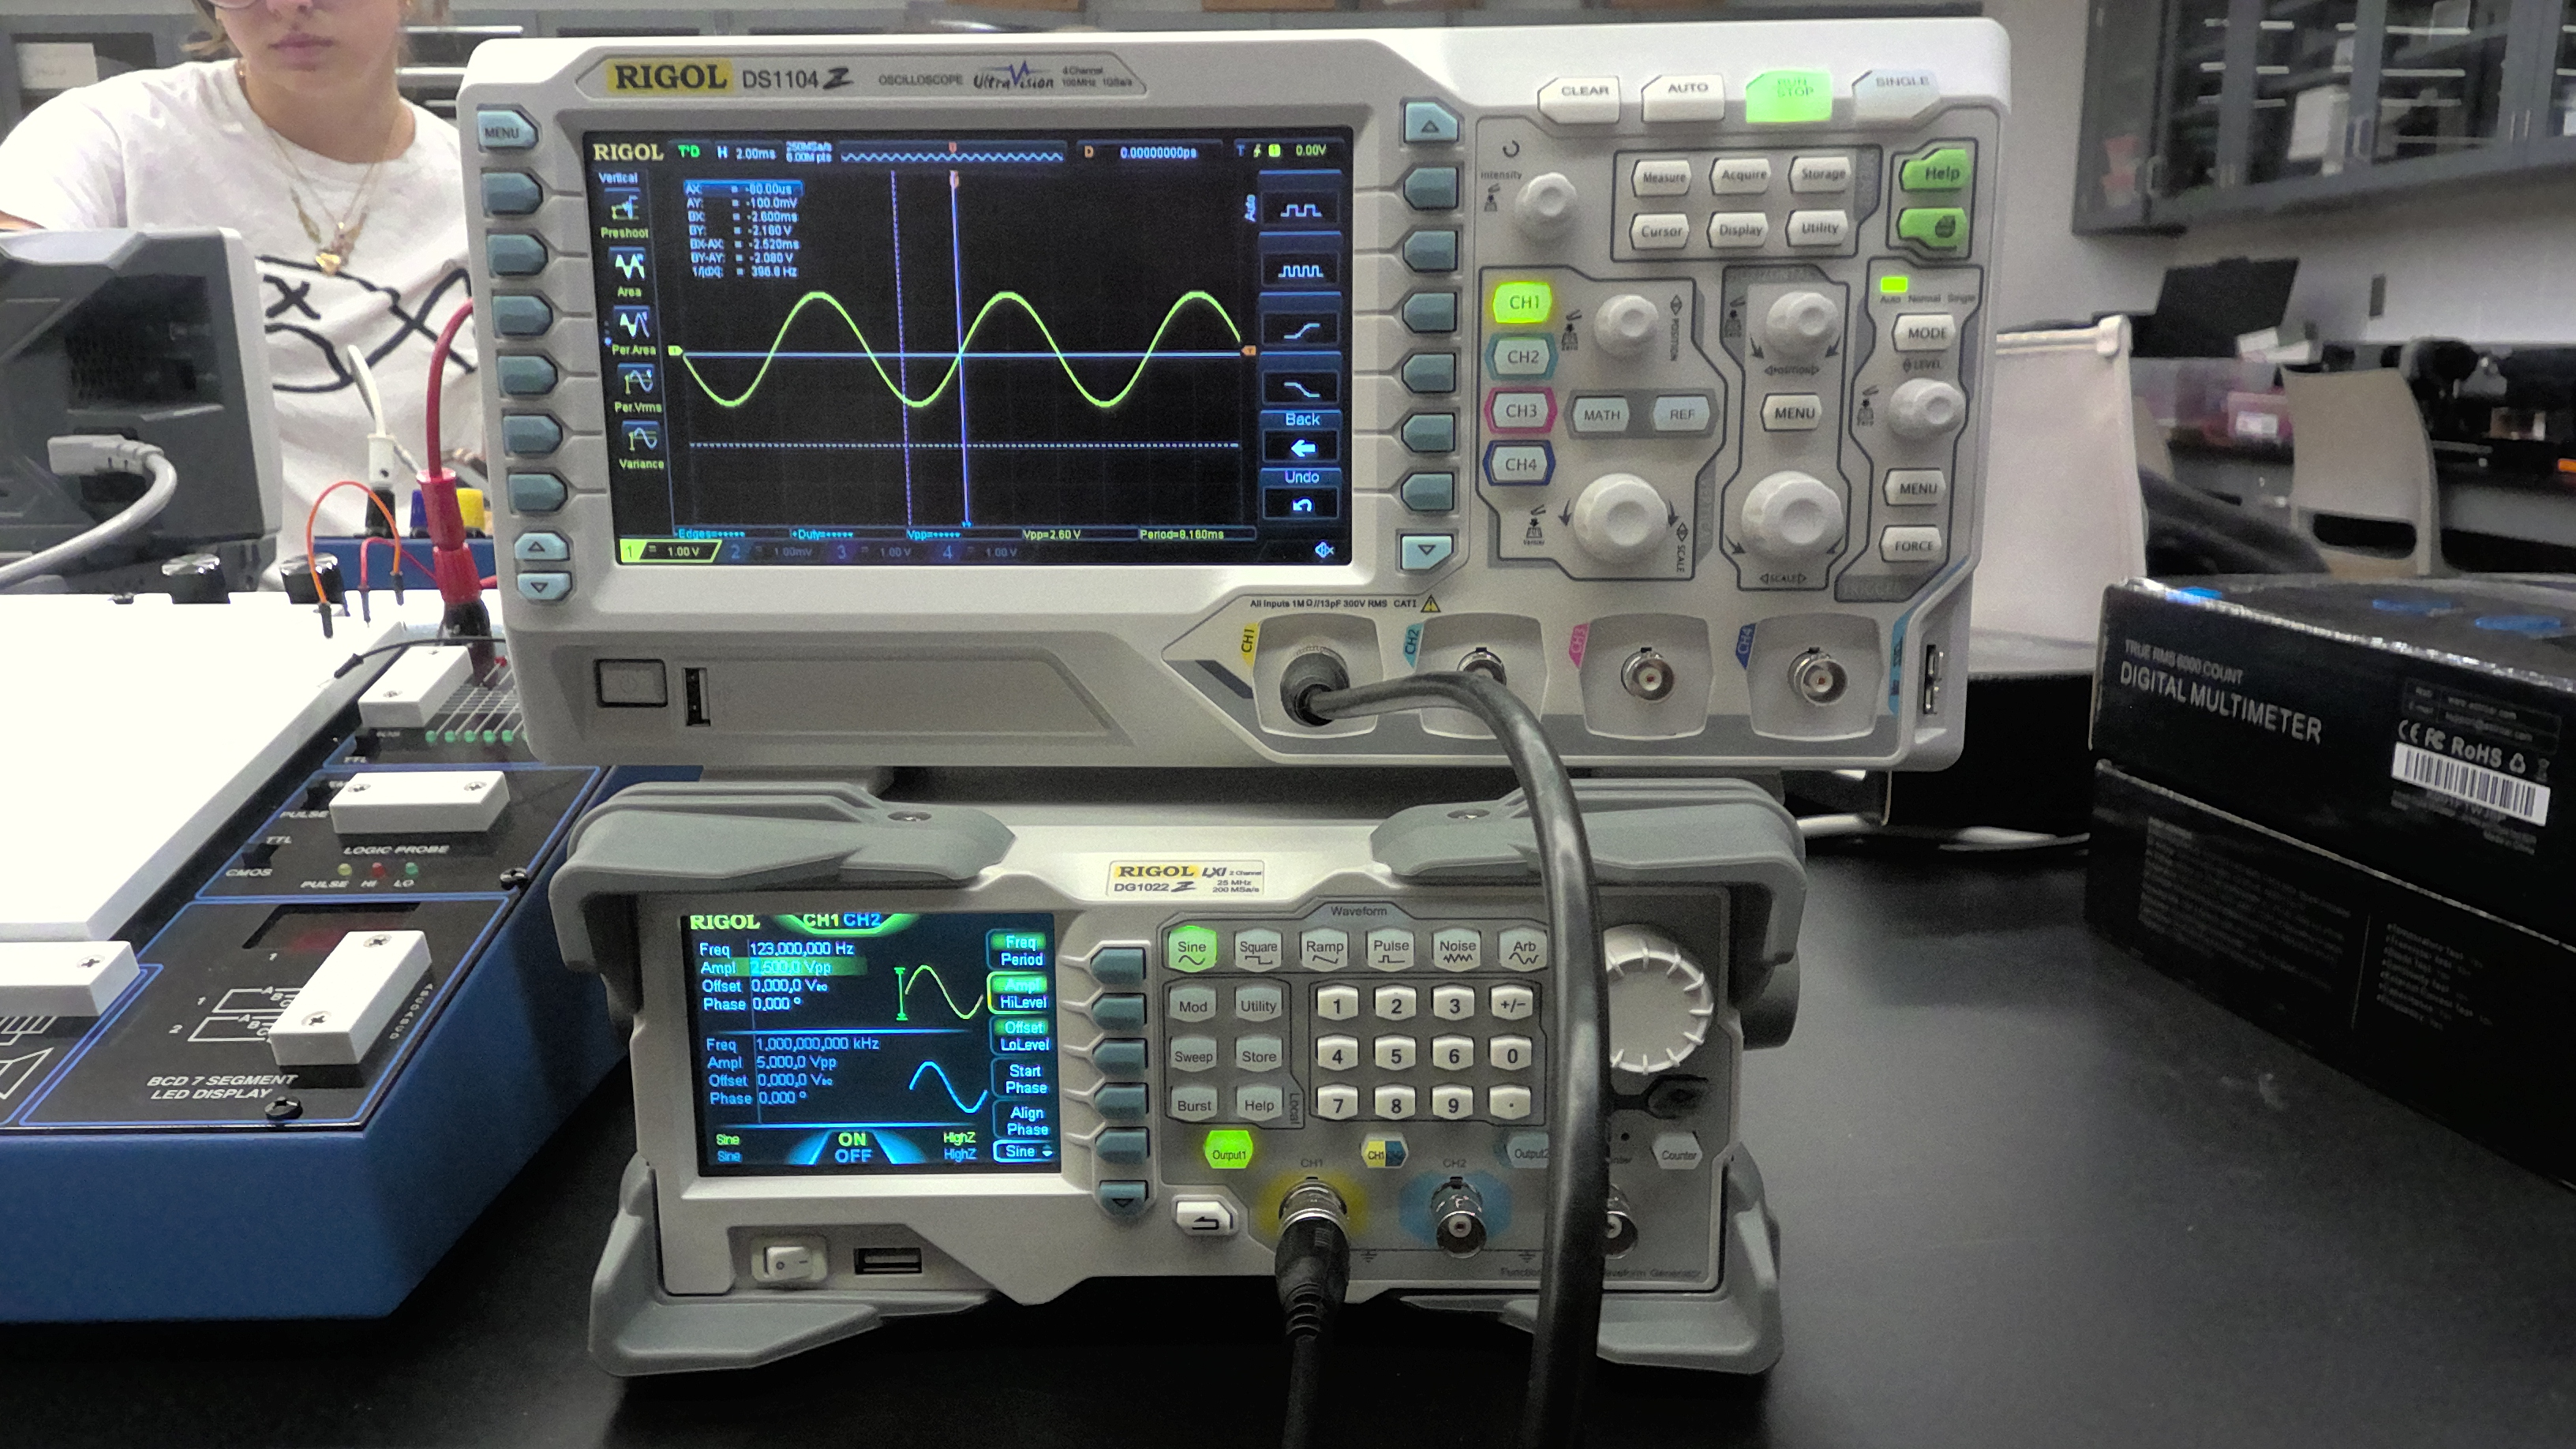
\includegraphics[width=0.5\textwidth]{WIN_20240927_13_48_12_Pro.jpg} %crop
        \caption{The oscilloscope (top) connected to the function generator (bottom) via coaxial cable.}
        \label{oscnfunc1}
    \end{figure}

    \subsection{Oscilloscope basics}
        In order to generate a signal to view in the oscilloscope, the function generator was configured as shown in figure \ref{funcgen1} to produce a 2.5 V, 123 Hz sine wave.

        \begin{figure}
            \centering
            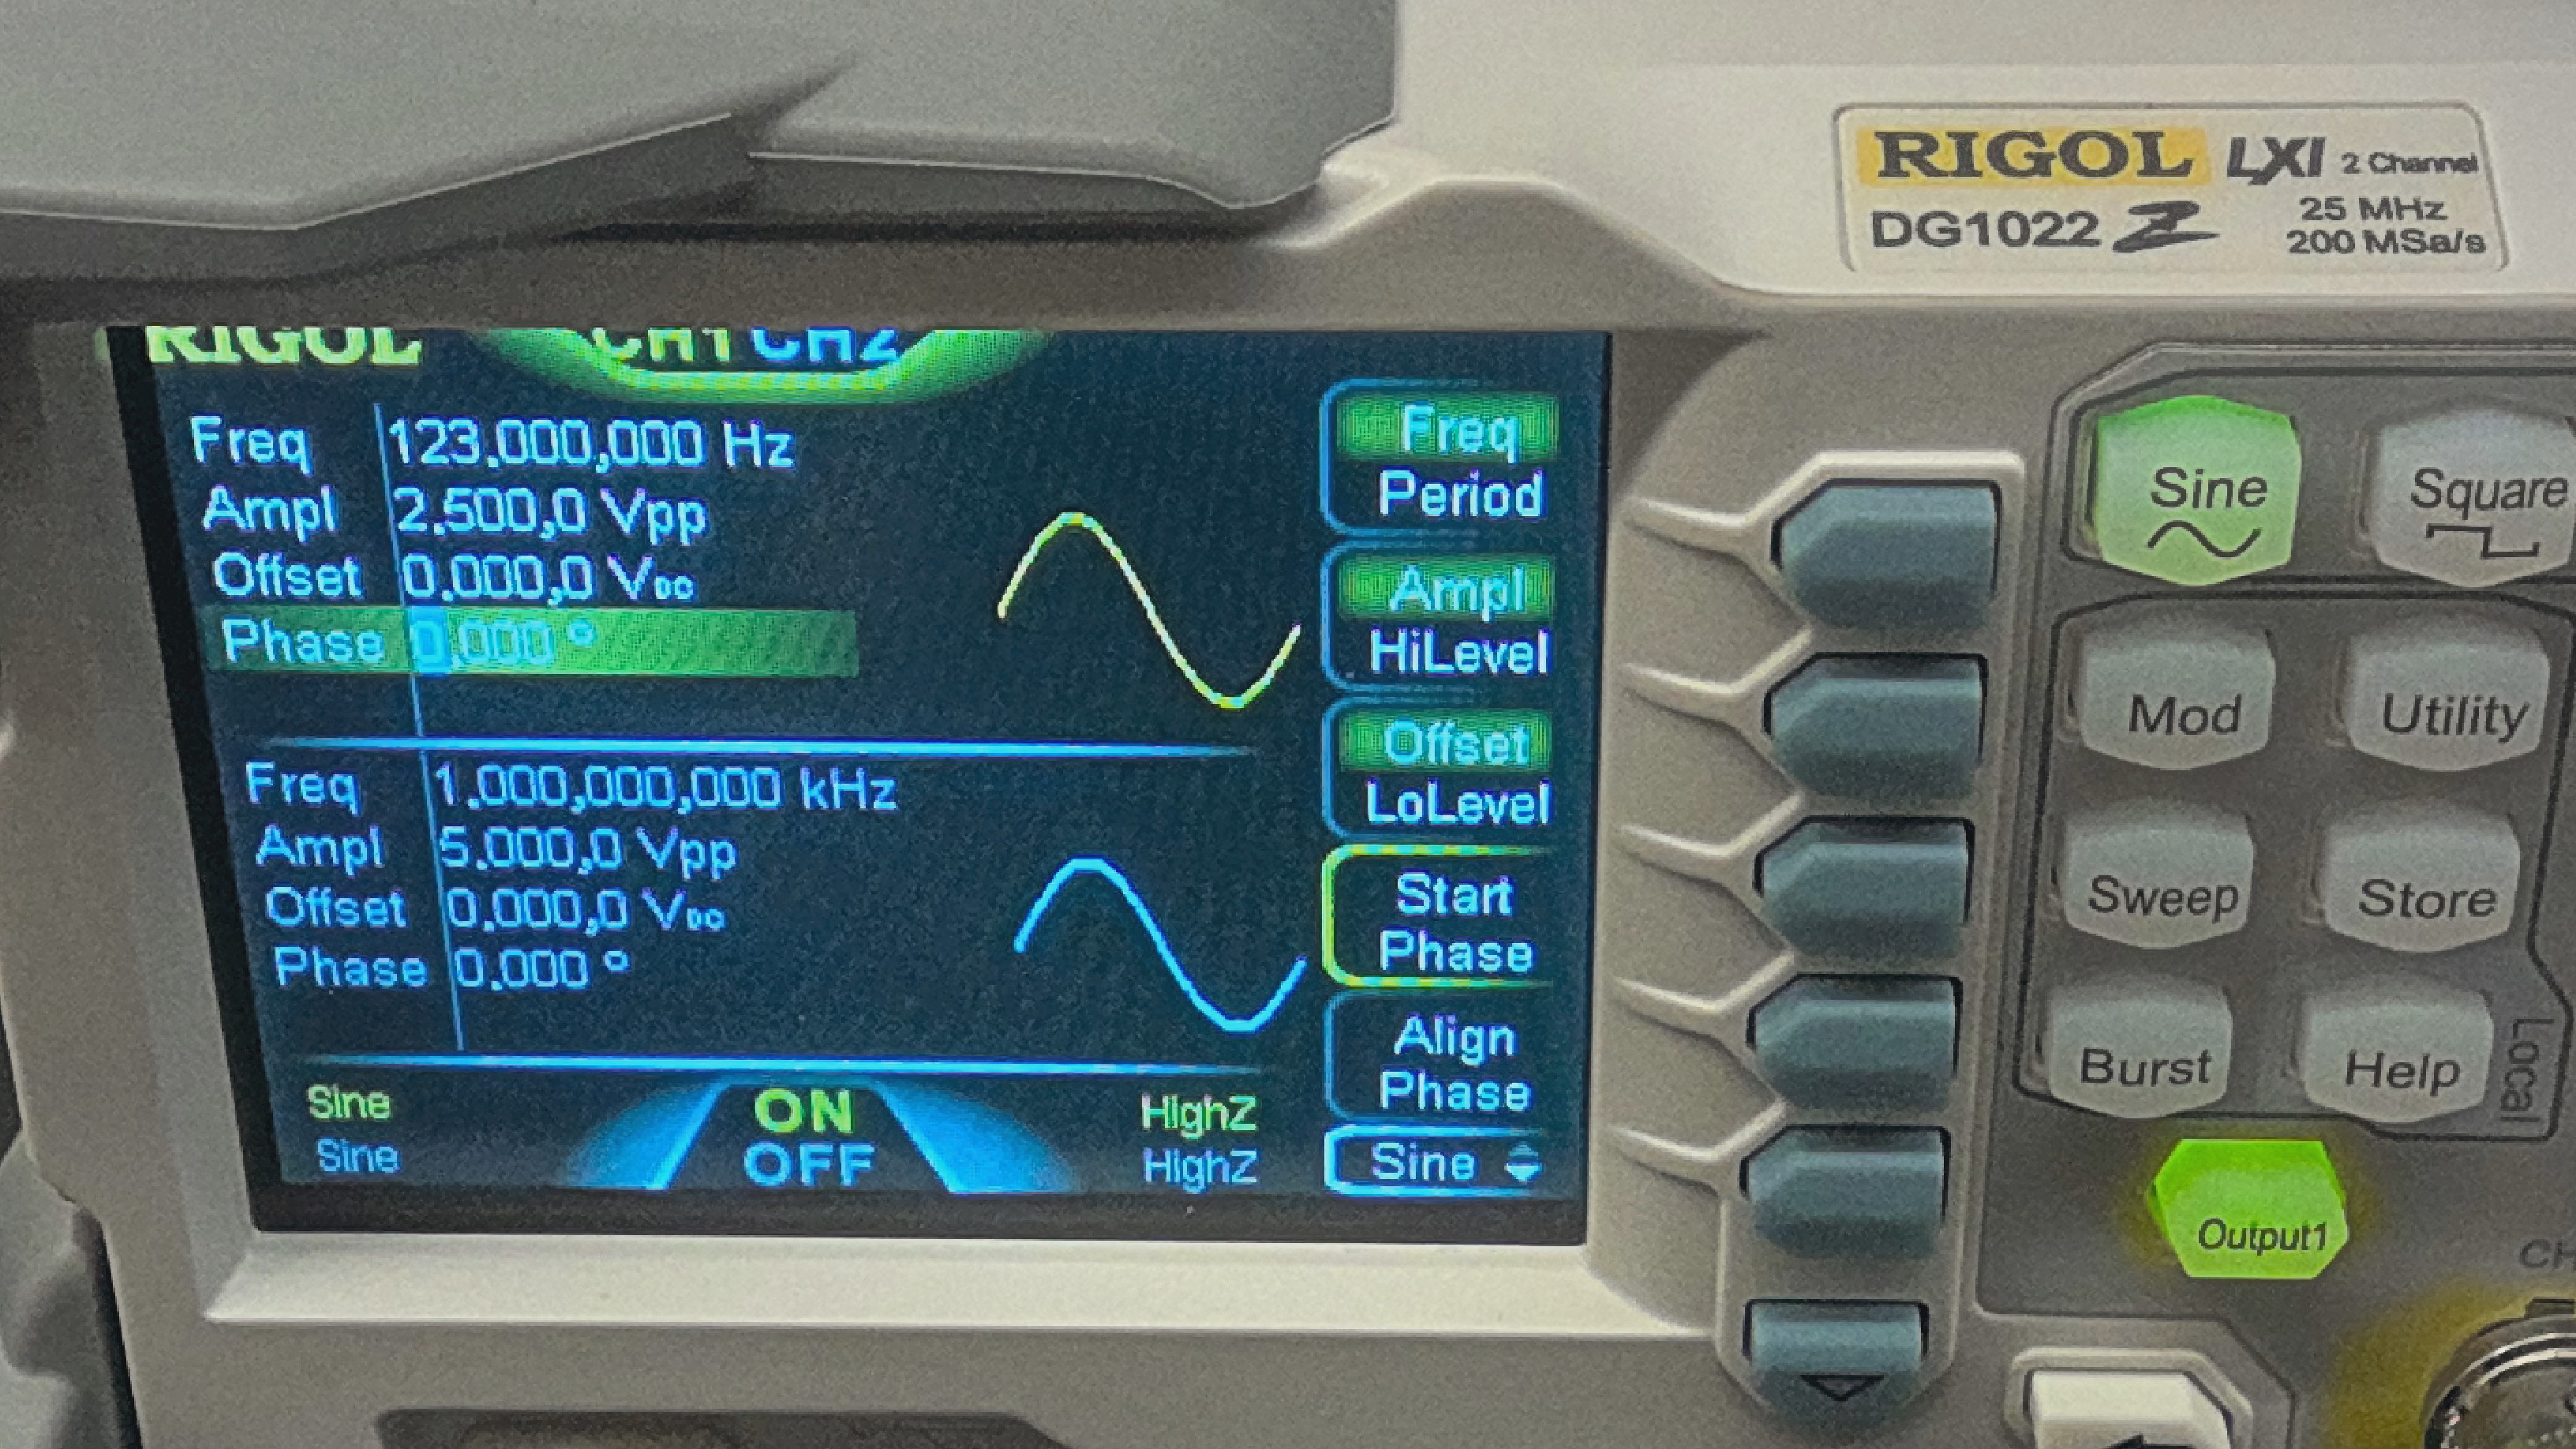
\includegraphics[width=0.5\textwidth]{WIN_20240927_13_51_59_Pro.jpg}
            \caption{The interface of the function generator.}
            \label{funcgen1}
        \end{figure}

        % MORE


    \subsection{Charging \& discharging of a capacitor}
        Thus far, only the output of the function generator had been investigated using the oscilloscope. In actual practice, oscilloscopes are used in a similar manner to a voltmeter---that is, they are connected in parallel to the component across which the voltage is to be measured. \\% grammar?
        For this portion of the experiment, a circuit would be constructed on a breadboard consisting of two parallel LEDs, a 997 $\Omega$ resistor, and 100.9 nF capacitor in series with the output of the function generator as shown in figure \ref{circuitry}.
        The function generator was configured to produce an 8 V, 500 Hz square wave which was output to both the circuit \& the first channel of the oscilloscope by means of a Tee-splitter.
        Across the capacitor was also placed a probe, which was connected to the second channel of the oscilloscope.

        \begin{figure}
            \centering
            \begin{minipage}{0.3\textwidth}
                    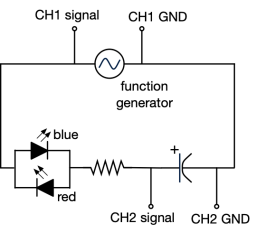
\includegraphics[width=0.8\linewidth]{g115.png}
                    \caption{Idealized circuit diagram.}
            \end{minipage}
            \begin{minipage}{0.3\textwidth}
                    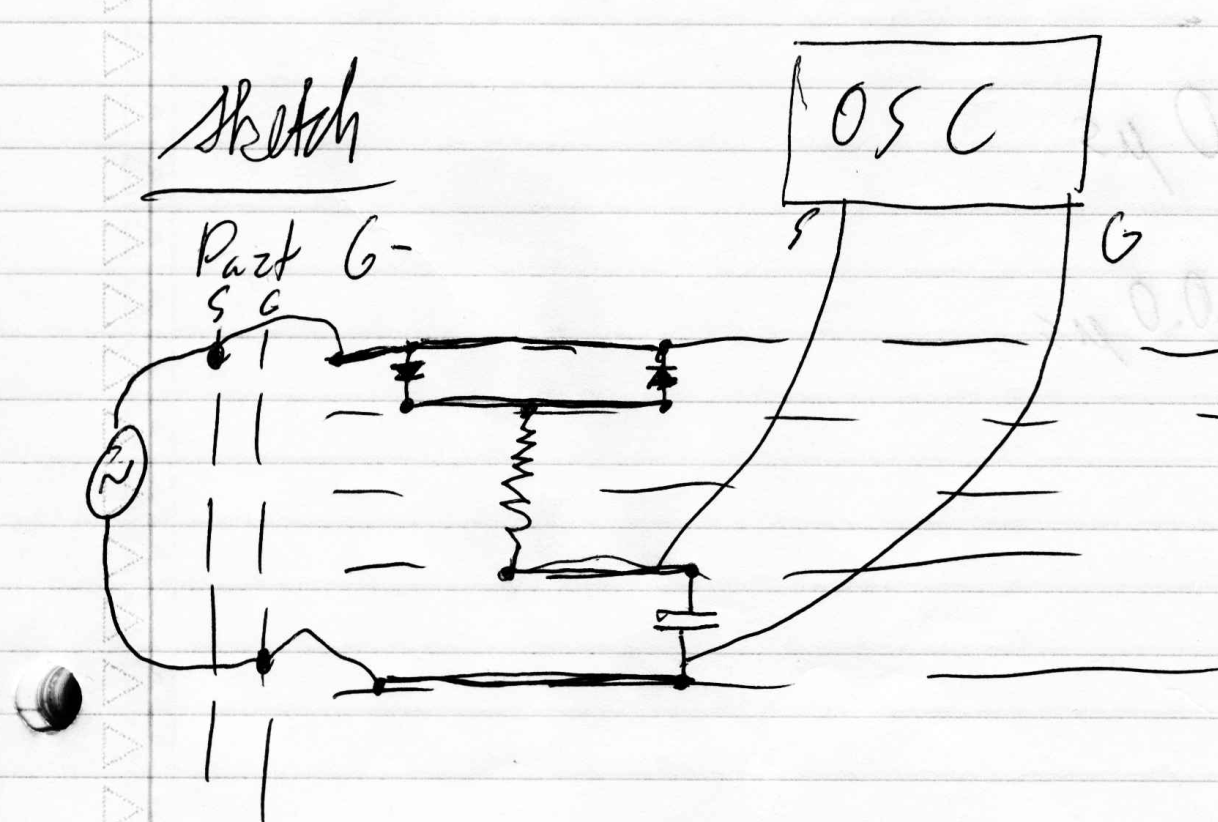
\includegraphics[width=0.8\linewidth]{breadboard.png}
                    \caption{Rough sketch of breadboard circuit.}
            \end{minipage}
            \begin{minipage}{0.3\textwidth}
                    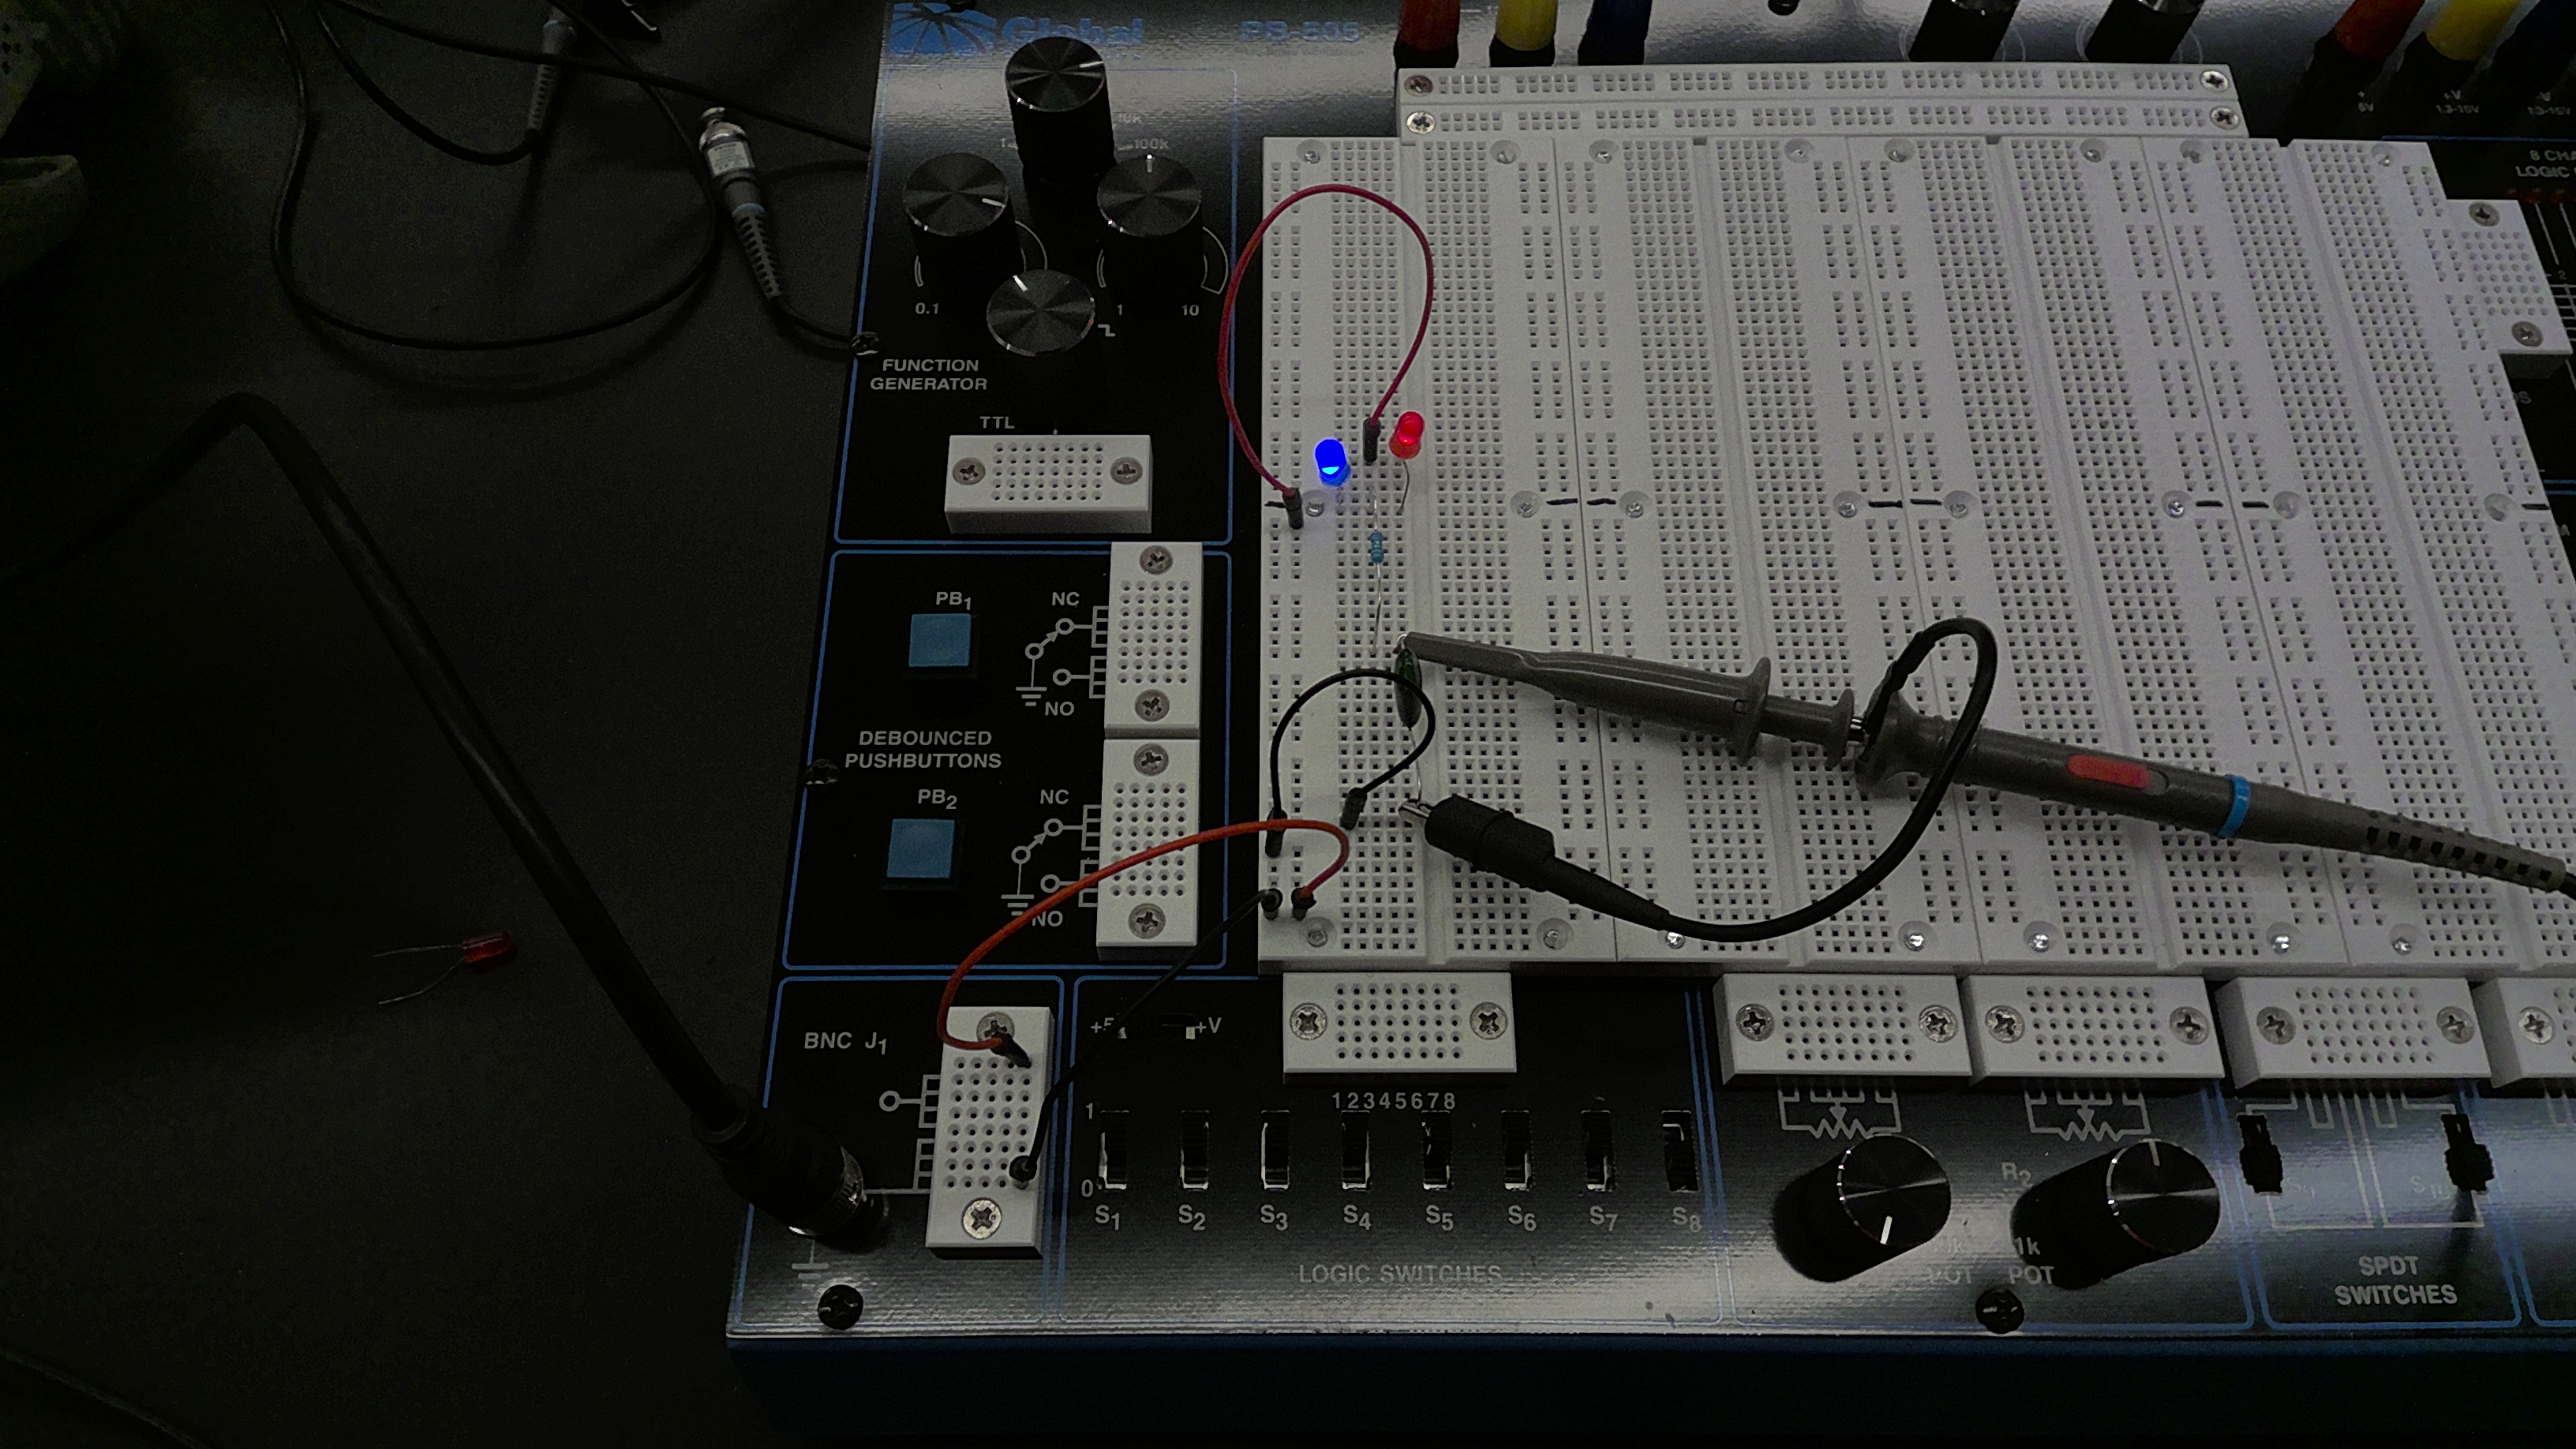
\includegraphics[width=0.8\linewidth]{circuit.jpg}
                    \caption{Circuit as assembled on breadboard.}
            \end{minipage}
        \end{figure}



\section{Exercises}


\section{Results}
\begin{table}
    
\end{table}

\section{Conclusion}

\end{document}